\newpage
\section{Đề thi Đại số}
\begin{tcolorbox}[title=\textbf{Bài toán B.1.}]
    Cho $a$ là một số thực, $A$ là ma trận phụ thuộc vào $a$
    $$A = \begin{pmatrix}[]{cccc}
        1 & a+1 & a+2 & 0 \\
        a+3 & 1 & 0 & a+2 \\
        a+2 & 0 & 1 & a+1 \\
        0 & a+2 & a+3 & 1 
    \end{pmatrix}.$$

    \begin{enumerate}
        \item[(a)] Tìm hạng của ma trận $A$ khi $a = -1$.
        \item[(b)] Tìm tất cả các số thực $a$ sao cho $A$ có định thức dương.
        \item[(c)] Biện luận số chiều của không gian nghiệm của hệ phương trình tuyến tính $AX = 0$ theo $a$ (ở đây $X$ là vector cột ứng với các tọa độ lần lượt là $x,\,y,\,z,\,t$). 
    \end{enumerate}
\end{tcolorbox}

\textbf{Lời giải.}

\begin{enumerate}
    \item[(a)] {
        Khi $a = -1$ thì 
        \begin{align*}
            A 
            & = \begin{pmatrix}[]{cccc}
                1 & 0 & 1 & 0 \\
                2 & 1 & 0 & 1 \\
                1 & 0 & 1 & 0 \\
                0 & 1 & 2 & 1 
            \end{pmatrix} \sim \begin{pmatrix}[]{cccc}
                1 & 0 & 1 & 0 \\
                2 & 1 & 0 & 1 \\
                0 & 1 & 2 & 1 \\
                1 & 0 & 1 & 0 
            \end{pmatrix} \sim \begin{pmatrix}[]{cccc}
                1 & 0 & 1 & 0 \\
                0 & 1 & -2 & 1 \\
                0 & 1 & 2 & 1 \\
                0 & 0 & 0 & 0 
            \end{pmatrix} \sim \begin{pmatrix}[]{cccc}
                1 & 0 & 1 & 0 \\
                0 & 1 & -2 & 1 \\
                0 & 0 & 4 & 0 \\
                0 & 0 & 0 & 0 
            \end{pmatrix}.
        \end{align*}

        Từ đây suy ra $\text{r}(A) = 3$.
    }
    \item[(b)] {
        Theo khai triển Laplace, ta có 

        \begin{align*}
            \det (A) 
            & = \begin{vmatrix}[]{ccc}
                1 & 0 & a+2 \\
                0 & 1 & a+1 \\
                a+2 & a+3 & 1 
            \end{vmatrix} - (a+1)\begin{vmatrix}[]{ccc}
                a+3 & 0 & a+2 \\
                a+2 & 1 & a+1 \\
                0 & a+3 & 1 
            \end{vmatrix} + (a+2)\begin{vmatrix}[]{ccc}
                a+3 & 1 & a+2 \\
                a+2 & 0 & a+1 \\
                0 & a+2 & 1 
            \end{vmatrix} \allowdisplaybreaks \\ 
            & = \left(\begin{vmatrix}[]{cc}
                1 & a+1 \\
                a+3 & 1 
            \end{vmatrix} + (a+2)\begin{vmatrix}[]{cc}
                0 & 1 \\
                a+2 & a+3 
            \end{vmatrix}\right) \\
            & \quad - (a+1)\left(\begin{vmatrix}[]{cc}
                a+3 & 0 \\
                a+2 & 1 
            \end{vmatrix} - (a+3)\begin{vmatrix}[]{cc}
                a+3 & a+2 \\
                a+2 & a+1 
            \end{vmatrix}\right) \allowdisplaybreaks \\
            & \quad + (a+2)\left(\begin{vmatrix}[]{cc}
                a+3 & 1 \\
                a+2 & 0 
            \end{vmatrix} - (a+2)\begin{vmatrix}[]{cc}
                a+3 & a+2 \\
                a+2 & a+1 
            \end{vmatrix}\right) \\   
            & = \Big(1-(a+3)(a+1) - (a+2)^2\Big) - (a+1)(a+3) - (a+2)^2 \\ 
            & \quad + \Big((a+1)(a+3) - (a+2)^2\Big)\begin{vmatrix}[]{cc}
                a+3 & a+2 \\
                a+2 & a+1 
            \end{vmatrix} \\
            & = -4a^2 - 16a - 13 - \begin{vmatrix}[]{cc}
                a+3 & a+2 \\
                a+2 & a+1 
            \end{vmatrix} \\
            & = -4a^2 - 16a - 12 \\
            & = -4(a+1)(a+3).
        \end{align*}

        Như vậy $\det (A) > 0 \iff -4(a+1)(a+3) > 0 \iff -3 < a < -1$.
    }
    \item[(c)] {
        Với $a = -1$, theo câu (a) ta có $\text{r}(A) = 3$ nên số chiều của không gian nghiệm bằng $4 - \text{r}(A) = 1$.

        Với $a = -3$, ta có $$A = \begin{pmatrix}[]{cccc}
            1 & -2 & -1 & 0 \\
            0 & 1 & 0 & -1 \\
            -1 & 0 & 1 & -2 \\
            0 & -1 & 0 & 1 
        \end{pmatrix} \sim \begin{pmatrix}[]{cccc}
            1 & -2 & -1 & 0 \\
            0 & 1 & 0 & -1 \\
            0 & -2 & 0 & -2 \\
            0 & 0 & 0 & 0 
        \end{pmatrix} \sim \begin{pmatrix}[]{cccc}
            1 & -2 & -1 & 0 \\
            0 & 1 & 0 & -1 \\
            0 & 0 & 0 & -4 \\
            0 & 0 & 0 & 0 
        \end{pmatrix},$$ từ đây suy ra $\text{r}(A) = 3$ nên số chiều của không gian nghiệm bằng $4 - \text{r}(A) = 1$.

        Với $a \ne -1,\,-3$ thì $\det (A) \ne 0$ nên hệ phương trình $AX = 0$ có nghiệm duy nhất nên số chiều của không gian nghiệm bằng 0.
    }
\end{enumerate}

\textbf{Nhận xét. }Đây là một bài toán cơ bản về ma trận. Câu (a) và (b) yêu cầu các tính toán cơ bản về định thức và hạng của ma trận. Câu (c) liên quan đến tính chất số chiều của không gian nghiệm của phương trình thuần nhất bằng số ẩn tự do, bằng với số hàng toàn 0 khi đưa ma trận hệ số về ma trận bậc thang, và bằng hiệu giữa số ẩn và hạng của ma trận hệ số.

\begin{tcolorbox}[title=\textbf{Bài toán B.2.}]
    Cho $A,\,B$ là hai ma trận vuông $$A = \begin{pmatrix}[]{cc}
        0 & 2 \\
        1 & 0 
    \end{pmatrix},\,B = \begin{pmatrix}[]{cc}
        0 & -2 \\
        -1 & 0 
    \end{pmatrix}.$$

    \begin{enumerate}
        \item[(a)] Tìm một ma trận thực $P$ có cấp bằng 2, sao cho $P^{-1}AP$ là ma trận đường chéo.
        \item[(b)] Tìm một ma trận thực $R$ có cấp bằng 2, định thức bằng 1, sao cho $R^{-1}AR = B$.
    \end{enumerate}
\end{tcolorbox}

\textbf{Lời giải.}

\begin{enumerate}
    \item[(a)] {
        Xét ma trận $P = \begin{pmatrix}[]{cc}
            \sqrt{2} & -\sqrt{2} \\
            1 & 1
        \end{pmatrix}$ có $\det (P) = 2\sqrt{2} \ne 0$ nên $P$ khả nghịch.
        
        Khi đó $$P^{-1} = \dfrac{1}{\det (P)} \cdot \text{adj}(P) = \dfrac{1}{2\sqrt{2}}\begin{pmatrix}[]{cc}
            1 & \sqrt{2} \\
            -1 & \sqrt{2} 
        \end{pmatrix},$$ trong đó $\text{adj}(P)$ là ma trận phụ hợp của ma trận $P$. 

        Kiểm tra bằng phép nhân ma trận, ta thấy $$P^{-1}AP = \begin{pmatrix}[]{cc}
            \sqrt{2} & 0 \\
            0 & -\sqrt{2} 
        \end{pmatrix}$$ là ma trận đường chéo.
    }
    \item[(b)] {
        Xét ma trận $Q = \begin{pmatrix}[]{cc}
            1 & -2 \\ 
            1 & -1
        \end{pmatrix}$ có $\det (Q) = 1 \ne 0$ nên $Q$ khả nghịch.
        
        Khi đó $$Q^{-1} = \dfrac{1}{\det (Q)} \cdot \text{adj}(Q) = \begin{pmatrix}[]{cc}
            -1 & 2 \\
            -1 & 1
        \end{pmatrix},$$ trong đó $\text{adj}(Q)$ là ma trận phụ hợp của ma trận $Q$. 

        Kiểm tra bằng phép nhân ma trận, ta thấy $$Q^{-1}AQ = \begin{pmatrix}[]{cc}
            0 & -2 \\
            -1 & 0 
        \end{pmatrix} = B.$$
    } 
\end{enumerate}

\textbf{Nhận xét. }Câu (a) là một bài toán chéo hóa ma trận cơ bản. Câu (b) giải được bằng cách đồng nhất hệ số và giải hệ phương trình. Ma trận $Q$ cần tìm có dạng tổng quát $\begin{pmatrix}[]{cc}
    a & b \\
    c & d 
\end{pmatrix}$, khi đó điều kiện đầu tiên là $\det(Q) = 1$ hay $ad - bc = 1$. Ngoài ra, $Q^{-1} = \dfrac{1}{\det (Q)} \cdot \text{adj}(Q) = \text{adj}(Q) = \begin{pmatrix}[]{cc}
    d & -b \\
    -c & a 
\end{pmatrix}$. Khi đó bằng phép nhân ma trận, ta có $Q^{-1}AQ = \begin{pmatrix}[]{cc}
    2cd-ab & 2d^2-b^2 \\
    a^2-2c^2 & ab-2cd 
\end{pmatrix}$ nên từ đó ta phải có $$\begin{pmatrix}[]{cc}
    2cd-ab & 2d^2-b^2 \\
    a^2-2c^2 & ab-2cd 
\end{pmatrix} = \begin{pmatrix}[]{cc}
    0 & -2 \\
    -1 & 0 
\end{pmatrix}.$$ 

Ta chọn $a,\,b,\,c,\,d$ thỏa mãn hệ phương trình $$\begin{cases}
    ad - bc = 1 \\
    2cd - ab = 0 \\
    2d^2 - b^2 = -2 \\
    a^2 - 2c^2 = -1 \\
    ad - 2cd = 0
\end{cases},$$
từ đó tìm được một bộ $(a,\,b,\,c,\,d)$ thỏa mãn hệ phương trình trên là $(1,\,-2,\,1,\,-1)$.

\begin{tcolorbox}[title=\textbf{Bài toán B.3.},breakable]
    Có 200 con muỗi trong một căn hộ gồm 4 phòng với hệ thống cửa nối các phòng như hình vẽ.

    \begin{center}
        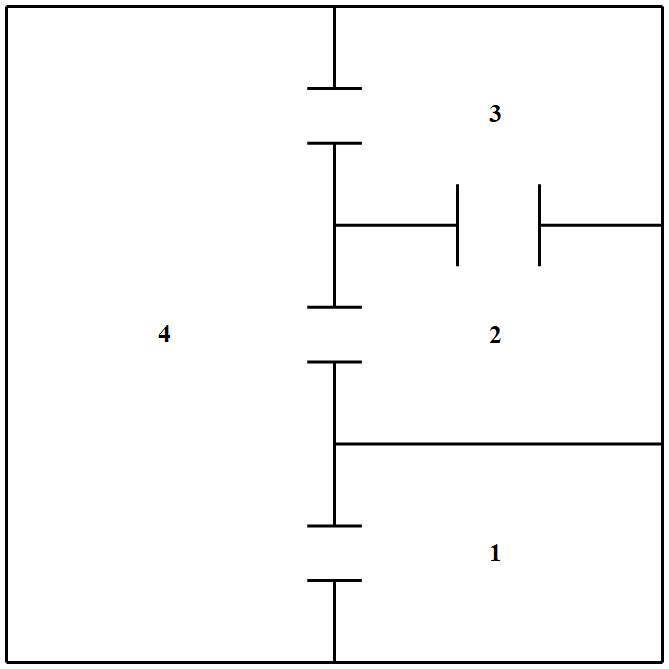
\includegraphics[width=0.5\textwidth]{Figures/01.png}
    \end{center}
    
    Biết rằng, mỗi phút, mỗi con muỗi chỉ ở lại trong phòng nó đang ở hoặc bay sang một phòng bên cạnh. Ngoài ra, người ta thống kê được rằng, với mỗi phòng, có 40\% số muỗi ở lại phòng đó, còn trong số muỗi bay ra khỏi phòng thì số lượng muỗi bay sang mỗi phòng bên cạnh đó là bằng nhau. Chẳng hạn, trong số các con muỗi bay từ phòng 3 sang phòng khác, thì có một nửa bay sang phòng 2, một nửa sang phòng 4.
    
    \begin{enumerate}
        % \begin{multicols}{2}
            \item {Giả sử sau một phút số muỗi ở các phòng 1, phòng 2, phòng 3 và phòng 4 tương ứng là 24, 50, 52 và 74. Tính số muỗi ở mỗi phòng tại thời điểm ban đầu.}
            \item {Gọi trạng thái ổn định là trạng thái mà kể từ đó trở đi số muỗi ở mỗi phòng đều không đổi. Tính số lượng muỗi tương ứng của mỗi phòng tại trạng thái ổn định đó.}         
        % \end{multicols}
    \end{enumerate}
\end{tcolorbox}

\textbf{Lời giải.}

Gọi $a_0,\,b_0,\,c_0,\,d_0$ lần lượt là số muỗi ban đầu của phòng 1, 2, 3, 4; $a_n,\,b_n,\,c_n,\,d_n$ lần lượt là số muỗi của phòng 1, 2, 3, 4 sau phút thứ $n$.

Nhận xét rằng sau mỗi phút, phòng 1 có 40\% số muỗi ở lại, cùng với 20\% số muỗi của phòng 4 bay ra (do 60\% số muỗi phòng 4 bay sang phòng 1, 2, 3) nên ta có phương trình $$a_{n+1} = 0.4a_n + 0.2d_n.$$

Lập luận tương tự, ta thiết lập được hệ phương trình $$\begin{cases}
    a_{n+1} = 0.4a_n + 0.2d_n \\
    b_{n+1} = 0.4b_n + 0.3c_n + 0.2d_n \\
    c_{n+1} = 0.3b_n + 0.4c_n + 0.2d_n \\
    d_{n+1} = 0.6a_n + 0.3b_n + 0.3c_n + 0.4d_n 
\end{cases}.$$

\begin{enumerate}
    \item[(a)] {
        Theo giả thiết, ta có 
        $$\begin{cases}
            0.4a_0 + 0.2d_0 = 24 \\
            0.4b_0 + 0.3c_0 + 0.2d_0 = 50 \\
            0.3b_0 + 0.4c_0 + 0.2d_0 = 52 \\
            0.6a_0 + 0.3b_0 + 0.3c_0 + 0.4d_0 = 74
        \end{cases}.$$

        Xét ma trận bổ sung và thực hiện biến đổi sơ cấp theo dòng 

        \begin{align*}
            \begin{pmatrix}[]{cccc|c}
                0.4 & 0 & 0 & 0.2 & 24 \\
                0 & 0.4 & 0.3 & 0.2 & 50 \\
                0 & 0.3 & 0.4 & 0.2 & 52 \\
                0.6 & 0.3 & 0.3 & 0.4 & 74 
            \end{pmatrix} & \sim \begin{pmatrix}[]{cccc|c}
                0.4 & 0 & 0 & 0.2 & 24 \\
                0 & 0.4 & 0.3 & 0.2 & 50 \\
                0 & 0.3 & 0.4 & 0.2 & 52 \\
                0 & 0.3 & 0.3 & 0.1 & 38 
            \end{pmatrix} \sim \begin{pmatrix}[]{cccc|c}
                0.4 & 0 & 0 & 0.2 & 24 \\
                0 & 0.4 & 0.3 & 0.2 & 50 \\
                0 & 0 & 0.175 & 0.05 & 14.5 \\
                0 & 0 & 0.075 & -0.05 & 0.5 
            \end{pmatrix} \\ & \sim \begin{pmatrix}[]{cccc|c}
                0.4 & 0 & 0 & 0.2 & 24 \\
                0 & 0.4 & 0.3 & 0.2 & 50 \\
                0 & 0 & 0.175 & 0.05 & 14.5 \\
                0 & 0 & 0 & -1/14 & -40/7 
            \end{pmatrix}.
        \end{align*}

        Từ đó ta có được $(a_0,\,b_0,\,c_0,\,d_0) = (20,\,40,\,60,\,80)$.
    }
    \item[(b)] {Ở trạng thái ổn định, ta có $$\begin{cases}
        a_{n} = 0.4a_n + 0.2d_n \\
        b_{n} = 0.4b_n + 0.3c_n + 0.2d_n \\
        c_{n} = 0.3b_n + 0.4c_n + 0.2d_n \\
        d_{n} = 0.6a_n + 0.3b_n + 0.3c_n + 0.4d_n 
    \end{cases} \iff \begin{cases}
        0.6a_n - 0.2d_n = 0 \\
        0.6b_n - 0.3c_n - 0.2d_n = 0 \\
        0.3b_n - 0.6c_n + 0.2d_n = 0 \\
        0.6a_n + 0.3b_n + 0.3c_n - 0.6d_n = 0
    \end{cases}.$$
    
    Xét ma trận hệ số và biến đổi sơ cấp theo dòng
    
    \begin{align*}
        \begin{pmatrix}[]{cccc}
            0.6 & 0 & 0 & -0.2 \\
            0 & 0.6 & -0.3 & -0.2 \\
            0 & 0.3 & -0.6 & 0.2 \\
            0.6 & 0.3 & 0.3 & -0.6 
        \end{pmatrix} & \sim \begin{pmatrix}[]{cccc}
            0.6 & 0 & 0 & -0.2 \\
            0 & 0.6 & -0.3 & -0.2 \\
            0 & 0.3 & -0.6 & 0.2 \\
            0 & 0.3 & 0.3 & -0.4 
        \end{pmatrix} \sim \begin{pmatrix}[]{cccc}
            0.6 & 0 & 0 & -0.2 \\
            0 & 0.6 & -0.3 & -0.2 \\
            0 & 0 & -0.45 & 0.3 \\
            0 & 0 & 0.45 & -0.3 
        \end{pmatrix} \\ & \sim \begin{pmatrix}[]{cccc}
            0.6 & 0 & 0 & -0.2 \\
            0 & 0.6 & -0.3 & -0.2 \\
            0 & 0 & -0.45 & 0.3 \\
            0 & 0 & 0 & 0
        \end{pmatrix} \sim \begin{pmatrix}[]{cccc}
            1 & 0 & 0 & -1/3 \\
            0 & 1 & 0 & -2/3 \\
            0 & 0 & 1 & -2/3 \\
            0 & 0 & 0 & 0
        \end{pmatrix}.
    \end{align*}
    
    Từ đó nghiệm tổng quát của hệ phương trình trên là $(a_n,\,b_n,\,c_n,\,d_n) = \left(\dfrac{1}{3}a,\,\dfrac{2}{3}a,\,\dfrac{2}{3}a,\,a\right)$ với mọi số thực $a$. Mặc khác, vì tổng số muỗi trong các phòng không đổi và bằng $24 + 50 + 52 + 74 = 200$ nên $\dfrac{1}{3}a + \dfrac{2}{3}a + \dfrac{2}{3}a + a = 200$, kéo theo $a = 75$. Như vậy số muỗi ở trạng thái ổn định trong phòng 1, 2, 3, 4 lần lượt là 25, 50, 50, 75.}
\end{enumerate}

\textbf{Nhận xét. }Đây là một bài toán Xích Markov chuyển trạng thái cơ bản, mấu chốt là phân tích được các giả thiết của bài toán và suy ra được hệ phương trình truy hồi ở trên. Bài toán dạng này có thể còn có câu hỏi rằng sau $x$ phút (5 phút, 10 phút,...) số muỗi của mỗi phòng tương ứng là bao nhiêu? Để giải quyết bài toán dạng này, ta viết lại hệ phương trình dưới dạng phương trình ma trận như sau 
$$\begin{pmatrix}[]{c}
    a_{n+1} \\ b_{n+1} \\ c_{n+1} \\ d_{n+1}
\end{pmatrix} = \begin{pmatrix}[]{cccc}
    0.4 & 0 & 0 & 0.2 \\
    0 & 0.4 & 0.3 & 0.2 \\
    0 & 0 & 0.175 & 0.05 \\
    0 & 0 & 0 & -1/14 
\end{pmatrix}\begin{pmatrix}[]{c}
    a_{n} \\ b_{n} \\ c_{n} \\ d_{n}
\end{pmatrix} = A\begin{pmatrix}[]{c}
    a_{n} \\ b_{n} \\ c_{n} \\ d_{n}
\end{pmatrix}.$$

Tính số muỗi của từng phòng sau $x$ phút, tức cần tính $$\begin{pmatrix}[]{c}
    a_{x} \\ b_{x} \\ c_{x} \\ d_{x}
\end{pmatrix} = A\begin{pmatrix}[]{c}
    a_{x-1} \\ b_{x-1} \\ c_{x-1} \\ d_{x-1}
\end{pmatrix} = A^2\begin{pmatrix}[]{c}
    a_{x-2} \\ b_{x-2} \\ c_{x-2} \\ d_{x-2}
\end{pmatrix} = \cdots = A^x\begin{pmatrix}[]{c}
    a_{0} \\ b_{0} \\ c_{0} \\ d_{0}
\end{pmatrix},$$ đến đây quy về việc tính lũy thừa ma trận $A^x$ là xong.

\begin{tcolorbox}[title=\textbf{Bài toán B.4.},breakable]
    \begin{enumerate}
        \item[(a)] {Có bao nhiêu cách chọn ra 3 viên gạch, mỗi viên từ một hàng trong hình sau đây, sao cho không có hai viên gạch nào được lấy ra nằm kề nhau (hai viên gạch được gọi là kề nhau nếu có chung một phần của một cạnh)?
        
        \begin{center}
            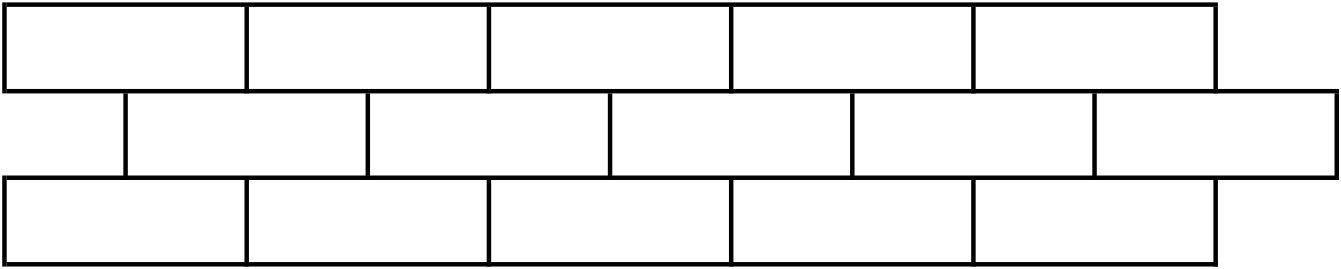
\includegraphics[width=0.6\textwidth]{Figures/02.png}
        \end{center}}
        \item[(b)] {Có bao nhiêu cách chọn ra 3 viên gạch, mỗi viên từ một hàng trong hình sau đây, sao cho không có hai viên gạch nào được lấy ra nằm kề nhau?
        
        \begin{center}
            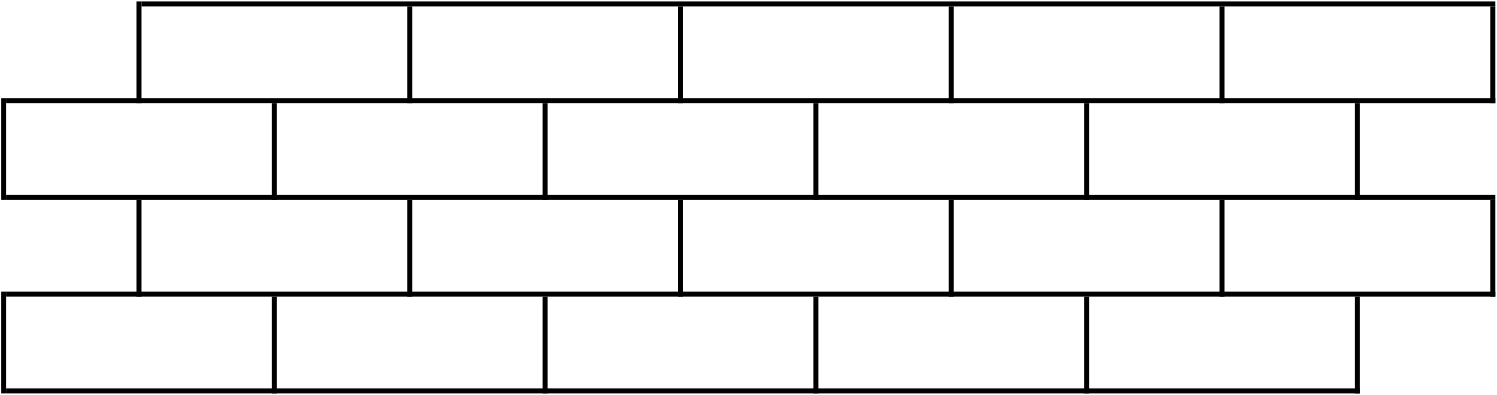
\includegraphics[width=0.6\textwidth]{Figures/03.png}
        \end{center}}
    \end{enumerate}
\end{tcolorbox}

\textbf{Lời giải. }

\begin{tcolorbox}[title=\textbf{Bài toán B.5.},breakable]
    Với $x,\,y,\,z$ là các số thực, đặt 
    $$A(x,\,y,\,z) = \det \begin{pmatrix}[]{ccc}
        x & y & z \\
        y & z & x \\
        z & x & y
    \end{pmatrix}$$
    \begin{enumerate}
        \item[(a)] {Tìm một không gian con $V$ của $\mathbb{R}^3$ với $\dim (V) = 2$ thỏa mãn $A(x,\,y,\,z)=0$ với mọi $(x,\,y,\,z) \in V$. Tìm một cơ sở của không gian $V$ vừa tìm được.}
        \item[(b)] {Tồn tại hay không các số nguyên $x,\,y,\,z$ sao cho $A(x,\,y,\,z) = 24$?}
    \end{enumerate}
\end{tcolorbox}

\textbf{Lời giải. }

\begin{enumerate}
    \item[(a)] {Theo khai triển Laplace, ta có 
    \begin{align*}
        A(x,\,y,\,z) 
        & = x\begin{vmatrix}[]{cc}
            z & x \\
            x & y
        \end{vmatrix} - y\begin{vmatrix}[]{cc}
            y & x \\
            z & y
        \end{vmatrix} + z\begin{vmatrix}[]{cc}
            y & z \\
            z & x
        \end{vmatrix} \\
        & = x(yz - x^2) - y(y^2 - zx) + z(xy - z^2) \\
        & = 3xyz - (x^3+y^3+z^3) \\
        & = (x + y + z)(xy + yz + zx - x^2 - y^2 - z^2).
    \end{align*}

    Ta có $$A(x,\,y,\,z) = 0 \iff \left[\begin{matrix}[]{l}
        x + y + z = 0 \\ xy + yz + zx - x^2 - y^2 - z^2 = 0
    \end{matrix} \right.$$

    Nhận xét rằng $xy + yz + zx - x^2 - y^2 - z^2 = 0\iff (x-y)^2 + (y-z)^2 + (z-x)^2 = 0 \iff x = y = z$ nên để không gian con $V$ cần tìm có $\dim(V) = 2$ thì $V$ là không gian nghiệm của phương trình $x + y + z = 0$. Phương trình có nghiệm tổng quát $(x,\,y,\,z) = (-y-z,\,y,\,z) = y(-1,\,1,\,0) + z(-1,\,0,\,1)$ với mọi $y,\,z \in \mathbb{R}$ nên $V$ có một cơ sở là $\left\{(-1,\,1,\,0),\,(-1,\,0,\,1)\right\}$.
    }
    \item[(b)] {Giả sử tồn tại các số nguyên $x,\,y,\,z$ thỏa mãn $A(x,\,y,\,z) = 24$ hay 
    \begin{align*}
        & (x + y + z)(xy + yz + zx - x^2 - y^2 - z^2) = 24 \\
        \iff & (x + y + z)\left(3(xy+yz+zx) - (x+y+z)^2\right) = 24 \\
        \iff & 3(x+y+z)(xy+yz+zx) - (x+y+z)^3 = 24.
    \end{align*}

    Vì 24 chia hết cho 3 nên vế trái cũng phải chia hết cho 3, kéo theo $(x+y+z)^3$ phải chia hết cho 3 hay $x+y+z$ chia hết cho 3. Khi đó $3(xy+yz+zx)-(x+y+z)^2$ chia hết cho 3, kéo theo $(x + y + z)\left(3(xy+yz+zx) - (x+y+z)^2\right)$ chia hết cho 9. Như vậy 24 cũng phải chia hết cho 9, thế nhưng đây là điều mâu thuẫn. Vậy điều giả sử là sai, hay không tồn tại $x,\,y,\,z$ để $A(x,\,y,\,z) = 24$.
    }
\end{enumerate}

\textbf{Nhận xét. }Mấu chốt trong bài toán này là tìm ra được đẳng thức $x^3 + y^3 + z^3 - 3xyz = (x+y+z)(x^2+y^2+z^2-xy-yz-zx)$. Đến đây nếu đã vững tính chất về không gian vector thì câu (a) được giải quyết gọn gàng. Câu (b) liên quan tới tính chia hết của số nguyên, mấu chốt là biến đổi $x^2+y^2+z^2-xy-yz-zx = (x+y+z)^2 - 3(xy+yz+zx)$ và nhận xét được $x+y+z$ chia hết cho 3. Nếu thay số 24 bởi một bội của 9, thì quy về giải phương trình nghiệm nguyên, bằng cách tách số ở vế phải thành tích của 2 số nguyên. 

Giả sử cần tìm $x,\,y,\,z$ để $A(x,\,y,\,z) = 9$. Để ý rằng $xy+yz+zx-x^2-y^2-z^2 = -\dfrac{1}{2}\left((x-y)^2 + (y-z)^2 + (z-x)^2\right) < 0$ và tương tự trên ta có được $x+y+z$ chia hết cho 3 nên ta chỉ xét trường hợp $x+y+z = xy+yz+zx-x^2-y^2-z^2 = -3$. Từ đây $3(xy+yz+zx)-(x+y+z)^2 = -3$ nên tính được $xy+yz+zx = 2$. Không mất tính tổng quát, giả sử $x$ là số nhỏ nhất trong ba số (trường hợp nếu $x+y+z > 0$ thì giả sử $x$ là số lớn nhất). Khi đó $x < 0$, vì nếu $x \leq 0$ thì $x + y + z \leq 0$ mâu thuẫn với $x + y + z = -3 < 0$. Như vậy ta đã thu hẹp được tập giá trị của $x$, đến đây xét từng giá trị $x$. Ứng với mỗi giá trị của $x$, từ $x + y + z = -3$ tính được $y + z$; từ $x(y+z) + yz=2$ tính được $yz$, từ đó tính được $xyz$. Khi có được $x+y+z,\,xy+yz+zx,\,xyz$ thì áp dụng Viete đảo để tìm $x,\,y,\,z$.

\begin{tcolorbox}[title=\textbf{Bài toán A.3.},breakable]
    Cho $P(x)$ là một đa thức với hệ số thực thỏa mãn $(x-1)P(x+1) = (x+2)P(x)$.
    \begin{enumerate}
        \item[(a)] {Chứng minh rằng $P(x)$ có ít nhất ba nghiệm thực phân biệt.}
        \item[(b)] {Tìm tất cả các đa thức $P(x)$ với hệ số thực thỏa mãn điều kiện trên.}
    \end{enumerate}
\end{tcolorbox}

\textbf{Lời giải. }

\begin{enumerate}
    \item[(a)] {
        Cho $x = -1$ thì có $P(-1) = 0$. Cho $x = 1$ thì có $P(1) = 0$. Cho $x = 0$ thì có $2P(0) = -P(1) = 0$ nên $P(0) = 0$. Như vậy $P(x)$ có ít nhất ba nghiệm thực là $-1,\,0,\,1$.
    } 
    \item[(b)] {Trước hết ta chứng minh bổ đề sau: Nếu đa thức $Q(x)$ hệ số thực thỏa mãn $Q(x) = Q(x+1)$ thì $Q(x) \equiv c$ với $c$ là hằng số.
    
    Thật vậy, giả sử $Q(x) = a_nx^n + a_{n-1}x^{n-1} + \ldots + a_1x + a_0\,(a_n \ne 0)$. Xét đa thức $T(x) = Q(x) - a_0$ thì ta có $T(0) = 0$. Mặt khác $T(x+1) = Q(x+1) - a_0 = Q(x) - a_0 = T(x)$ nên từ đó ta có $T(m) = T(m-1) = \ldots = T(1) = T(0) = 0$ với mọi $m$ nguyên dương nên $T(x)$ có vô số nghiệm, kéo theo $T(x) \equiv 0$. Như vậy $Q(x) \equiv a_0$ hay $Q(x) \equiv c$ với $c$ là hằng số.
    
    Quay trở lại bài toán, từ câu (a) $P(x)$ có ba nghiệm $-1,\,0,\,1$ nên $P(x) = x(x-1)(x+1)Q(x)$. Thay vào hệ thức ở đề bài, ta có $$(x-1)(x+1)x(x+2)Q(x+1) = (x+2)x(x-1)(x+1)Q(x) \iff Q(x+1) = Q(x).$$
    
    Áp dụng bổ đề vừa chứng minh, ta có $Q(x)\equiv c$ nên $P(x) \equiv cx(x-1)(x+1)$ với $c$ là hằng số thực.} 
\end{enumerate}

\textbf{Nhận xét. }Đây là một bài toán cơ bản về đa thức, sử dụng các tính chất về nghiệm của đa thức. Khi đề bài cho một hệ thức liên quan đến đa thức, một cách rất tự nhiên khi bắt tay vào làm là thế một vài giá trị đặc biệt để tìm ra tính chất nào đó của đa thức, mà ở đây là tìm ra được ba nghiệm của $P(x)$, chính là mấu chốt để giải quyết câu (b).

\begin{tcolorbox}[title=\textbf{Bài toán A.5.},breakable]
    Cặp ma trận thực, vuông cùng cấp $(A,\,B)$, được gọi là \textbf{tốt} nếu cả hai đều khả nghịch và thỏa mãn $AB-BA = B^2A$.
    \begin{enumerate}
        \item[(a)] {Chứng minh rằng nếu $(A,\,B)$ là một cặp ma trận tốt thì $$B = A^{-1}(B^2+B)A.$$}
        \item[(b)] {Tìm một cặp ma trận tốt $(A,\,B)$ với cấp của mỗi ma trận đều bằng 2.}
        \item[(c)] {Tìm tất cả các số nguyên dương $n$ sao cho tồn tại ít nhất một cặp ma trận tốt $(A,\,B)$ với cấp của mỗi ma trận đều bằng $n$.} 
    \end{enumerate}
\end{tcolorbox}

\textbf{Lời giải. }